% @author nicolas.guelfi
% @date Tue Nov 05 17:26:22 CET 2013
%-------------------------------------------------------------------------------
% Copyright (c) 2013 University of Luxembourg.
% All rights reserved. This program and the accompanying materials
% are made available under the terms of the Eclipse Public License v1.0
% which accompanies this distribution, and is available at
% http://www.eclipse.org/legal/epl-v10.html
% 
% Contributors:
%     Alfredo Capozucca - initial API and implementation
%     Benoit Ries - minor updates
%     Nicolas Guelfi - most content from messirbook
%-------------------------------------------------------------------------------
%%%%%%%%%%%%%%%%%%%%%%%%%%%%%%%%%%%%%%%%%%%%%%%%%%
\PassOptionsToPackage{usenames,svgnames,table}{xcolor}
\documentclass[graybox,envcountchap,sectrefs,11pt]{book} 
%%%%%%%%%%%%%%%%%%%%%%%%%%%%%%%%%%%%%%%%%%%%%%%%%%
%%% DO NOT CHANGE THE ORDER
\usepackage{./../lu.uni.lassy.excalibur.standard.report.libraries/styles/style-messir-common}
\usepackage{./../lu.uni.lassy.excalibur.standard.report.libraries/styles/style-messir-report-post}
%--------------------------------------------
% DOCUMENT BEGIN
%---------------------------------------- ----
\begin{document}

\newgeometry{textwidth=17cm,textheight=23.7cm} 


\newcommand{\msrReportType}{\emph{Report type: Simulation}} 
  

\definecolor{lightgray}{RGB}{201,201,201}
\definecolor{lightred}{RGB}{250,112,97}
\definecolor{lightgreen}{RGB}{179,250,140}

\definecolor{msrtextcl}{RGB}{0,0,0}
\definecolor{msrkeycl}{RGB}{127,0,85}
\definecolor{msrcmtcl}{RGB}{201,201,201}
\definecolor{keywordcolor}{RGB}{30,144,255}

\definecolor{aqua_blue}{RGB}{0,139,145}
\definecolor{dark_green}{RGB}{0,128,0}
\definecolor{dark_blue}{RGB}{45,45,138}

\definecolor{msrcolor01}{rgb}{0.96,0.59,0.48}
\definecolor{msrcolor02}{rgb}{1.00,0.97,0.60}
\definecolor{msrcolor03}{rgb}{0.51,0.79,0.61}
\definecolor{msrcolor04}{rgb}{0.43,0.81,0.96}
\definecolor{msrcolor05}{rgb}{0.52,0.58,0.79}
\definecolor{msrcolor06}{rgb}{0.96,0.61,0.76}
\definecolor{msrcolor07}{rgb}{0.98,0.68,0.51}
\definecolor{msrcolor08}{rgb}{0.77,0.88,0.61}
\definecolor{msrcolor09}{rgb}{0.49,0.66,0.85}
\definecolor{msrcolor10}{rgb}{0.96,0.60,0.62}
\definecolor{msrcolor11}{rgb}{0.64,0.83,0.61}
\definecolor{msrcolor12}{rgb}{0.63,0.53,0.75}
\definecolor{msrcolor13}{rgb}{0.99,0.78,0.54}
\definecolor{msrcolor14}{rgb}{0.53,0.51,0.74}
\definecolor{msrcolor15}{rgb}{0.48,0.80,0.79}
\definecolor{msrcolor16}{rgb}{0.74,0.55,0.75}
\definecolor{msrcolor17}{rgb}{0.90,0.79,0.08}
\definecolor{msrcolor18}{rgb}{1.00,1.00,0.00}
\definecolor{msrcolor19}{rgb}{1.00,0.00,0.50}

\definecolor{sepcolor000000}{rgb}{0, 0, 0}
\definecolor{sepcolor101010}{rgb}{0.10, 0.10, 0.10}
\definecolor{sepcolor202020}{rgb}{0.20, 0.20, 0.20}
\definecolor{sepcolor303030}{rgb}{0.30, 0.30, 0.30}
\definecolor{sepcolor404040}{rgb}{0.10, 0.10, 0.10}
\definecolor{sepcolor505050}{rgb}{0,1,.5}
\definecolor{sepcolor907908}{rgb}{0,1,.5}

\definecolor{sepregioncolor01}{rgb}{0.00,0.66,0.00}
\definecolor{sepregioncolor02}{rgb}{1.00,1.00,0.00}
\definecolor{sepregioncolor03}{rgb}{1.00,0.97,0.60}
\definecolor{sepregioncolor04}{rgb}{0.64,0.83,0.61}
\definecolor{sepregioncolor05}{rgb}{0.95,0.36,0.00}
\definecolor{sepregioncolor06}{rgb}{0.90,0.79,0.08}
\definecolor{sepregioncolor07}{rgb}{0.63,0.53,0.75}
\definecolor{sepregioncolor08}{rgb}{0.99,0.78,0.54}
\definecolor{sepregioncolor09}{rgb}{0.96,0.61,0.76}
\definecolor{sepregioncolor10}{rgb}{1.00,0.00,0.50}

\colorlet{msrcolorbrown}{red!40!black!80}


% Messir General
%----------------------------------------------------------

% quotePosition + quoteWidth + quotefillColor + quoteElement + quotedElement + allImageScale
\newcommand{\msrcallouted}[6]{
\scalebox{#1}{\parbox{\linewidth}{
  \begin{tikzpicture}
      \node [rectangle callout,callout relative pointer={#4},text width=#5,fill=#6,rounded corners] (tmpcall) at (0,0) {#3};
      \node at (tmpcall.pointer){#2};
  \end{tikzpicture}
}}
}

% Vresion wihtout scaling the quoted text
\pgfkeys{%
    /calloutquote/.cd,
    width/.code                   =  {\def\calloutquotewidth{#1}},
    position/.code                =  {\def\calloutquotepos{#1}}, 
    author/.code                  =  {\def\calloutquoteauthor{#1}},
    /calloutquote/.unknown/.code   =  {\let\searchname=\pgfkeyscurrentname
                                 \pgfkeysalso{\searchname/.try=#1,
    /tikz/\searchname/.retry=#1},\pgfkeysalso{\searchname/.try=#1,
                                  /pgf/\searchname/.retry=#1}}
                            }  

\newcommand\calloutquote[2][]{%
  \pgfqkeys{/calloutquote}{#1}
  \node [rectangle callout,callout relative pointer={\calloutquotepos},text width=\calloutquotewidth,/calloutquote/.cd,#1] (tmpcall) at (0,0) {#2};
  \node at (tmpcall.pointer){\calloutquoteauthor};    
}  
%----------------------------------------------------------
\newcommand{\msrTalkRD}[6]{
\freeblock{5}{#1}{#2}{
\begin{figure}
  \centering
  \includegraphics[width=#5]{images/various/descartes.pdf} 
\end{figure}
}
\freeblock{5}{#3}{#4}{
\scriptsize
\textit{#6}
}
}
\newcommand{\msrTalkGB}[6]{
\freeblock{5}{#1}{#2}{
\begin{figure}
  \centering
  \includegraphics[width=#5]{images/various/graham-bell.pdf} 
\end{figure}
}
\freeblock{5}{#3}{#4}{
\scriptsize
\textit{#6}
}
}
%----------------------------------------------------------

\newcommand{\msrQuestionSlide}[1]{
\begin{frame}[fragile]
\freeblock{5}{1}{4}{
\begin{figure}
  \centering
  \includegraphics[width=3cm]{images/various/3d-man-question-sit.pdf}
\end{figure}
}
\freeblock{10}{5}{3}{
\Large
\msrtxtclb{red}{\textit{#1}}
}
\end{frame}
}

%%%%%%%%%%%%%%%%%%%%%%%%%%%%%%%%%%%%%%%%%%%%%%%%%%%%%%%%%%
%%%%%%%%%%%%%%%%%%%%%%%%%%%%%%%%%%%%%%%%%%%%%%%%%%
%%% AUDIO
%%%%%%%%%%%%%%%%%%%%%%%%%%%%%%%%%%%%%%%%%%%%%%%%%%

\DeclareRobustCommand{\MyIncludeMedia}[5]{%
\addmediapath{#1}
\includemedia[
  flashvars={source=#2%
  &hideBar=true%
  &autoPlay=#3%
  },
  activate=pagevisible,
  noplaybutton,
  addresource=#2,
  transparent,
  passcontext
]{\includegraphics[width=.8cm]{#4}}{APlayer.swf}%
}

\DeclareRobustCommand{\slidesAudioModeChange}[1]
{\renewcommand{\slidesAudioMode}{#1}}

\DeclareRobustCommand{\slidesAudioHelp}{%
\IfSubStr{\slidesAudioMode}%
{remove}%
{}
{%
\pdfcomment[icon=Help,color=blue!10,open=false,subject={standard 14 fonts}]{Right clic on flag to have options !\\
Audio only available with Acrobat\ldots}%
}
}


\DeclareRobustCommand{\MyAudioButton}[3]{%
\IfSubStr{\slidesAudioMode}%
{remove}%
{}
{%
\IfSubStr{#1}{pause}{\def\MyAutoPlayMode{false}}{}%
\IfSubStr{#1}{\slidesAudioMode}{\def\MyAutoPlayMode{true}}{\def\MyAutoPlayMode{false}}%
\IfSubStr{#1}%
{fr}%
{\def\MyAudioIconPath{./../lu.uni.lassy.messir.common.slides/images/various/flag-audio-FR.pdf}}{}%
\IfSubStr{#1}%
{en}%
{\def\MyAudioIconPath{./../lu.uni.lassy.messir.common.slides/images/various/flag-audio-EN.pdf}}{}%
\IfSubStr{#1}%
{de}%
{\def\MyAudioIconPath{./../lu.uni.lassy.messir.common.slides/images/various/flag-audio-DE.pdf}}{}%
\IfSubStr{#1}%
{lu}%
{\def\MyAudioIconPath{./../lu.uni.lassy.messir.common.slides/images/various/flag-audio-LU.pdf}}{}%
\MyIncludeMedia{#2}{#3}{\MyAutoPlayMode}{\MyAudioIconPath}{#1}%
}
}
\makeatletter % we need to use kernel commands
\newcommand{\MyAudioBegin}{%
\begin{flushright}%
\setstretch{.3}
\@MyAudioOne%
}
\newcommand\@MyAudioOne{\@ifnextchar\stopaudio{\@MyAudioEnd}{\@MyAudioTwo}}

\newcommand\@MyAudioTwo[3]{%
\hspace*{-0.1cm}\@MyAudioThree{#1}{#2}{#3}%
\@MyAudioOne% restart the recursion
}
\newcommand\@MyAudioThree[3]{%
\MyAudioButton{#1}%
{#2}%
{#3}%
}
\newcommand\@MyAudioEnd[1]{% The argument is \stopaudio
\end{flushright}%
}
\makeatother

%%%%%%%%%%%%%%%%%%%%%%%%%%%%%%%%%%%%%%%%%%%%%%%%%%

\DeclareRobustCommand{\msrfigure}[4]{
\begin{figure}[!htbp]
\begin{center}
\scalebox{#1}{
\centering
{\begin{minipage}[c]{\linewidth}
\centering
#2
\end{minipage}
}}
\end{center}
\ifthenelse{\equal{#4}{}}
             {}
             {\caption{#4}}
\label{#3}
\end{figure}
}

\newcommand{\semitransp}[2][30]{\color{fg!#1}#2}
\newcommand*{\msrtechfont}{\fontfamily{ptm}\selectfont}

\DeclareRobustCommand{\msruml}{{\msrtechfont UML}~}
\DeclareRobustCommand{\msrocl}{{\msrtechfont OCL}~}
\DeclareRobustCommand{\msromg}{{\msrtechfont OMG}~}
\DeclareRobustCommand{\msrxtext}{{\msrtechfont Xtext}~}
\DeclareRobustCommand{\msremf}{{\msrtechfont EMF}~}
\DeclareRobustCommand{\msrcm}{\msrcode{{Concept Model}}~}

\DeclareRobustCommand{\msrapache}{{\msrtechfont Apache}~}
\DeclareRobustCommand{\msratlassian}{{\msrtechfont Atlassian}~}
\DeclareRobustCommand{\msrbamboo}{{\msrtechfont Bamboo}~}
\DeclareRobustCommand{\msrconfluence}{{\msrtechfont Confluence}~}
\DeclareRobustCommand{\msreclemma}{{\msrtechfont EclEmma}~}
\DeclareRobustCommand{\msreclipse}{{\msrtechfont Eclipse}~}
\DeclareRobustCommand{\msrsql}{{\msrtechfont SQL}~}
\DeclareRobustCommand{\msrjava}{{\msrtechfont Java}~}
\DeclareRobustCommand{\msrjavafx}{{\msrtechfont JavaFx}~}
\DeclareRobustCommand{\msrjira}{{\msrtechfont JIRA}~}
\DeclareRobustCommand{\msrjunit}{{\msrtechfont JUnit}~}
\DeclareRobustCommand{\msrlatex}{{\msrtechfont Latex}~}
\DeclareRobustCommand{\msrmaven}{{\msrtechfont Maven}~}
\DeclareRobustCommand{\msrmysql}{{\msrtechfont MySQL}~}
\DeclareRobustCommand{\msrocl}{{\msrtechfont OCL}~}
\DeclareRobustCommand{\msrpdf}{{\msrtechfont PDF}~} 
\DeclareRobustCommand{\msrsirius}{{\msrtechfont Sirius}~} 
\DeclareRobustCommand{\msrsvn}{{\msrtechfont SubVersioN}~}
\DeclareRobustCommand{\msrswtbot}{{\msrtechfont SWTbot}~}
\DeclareRobustCommand{\msrxtext}{{\msrtechfont Xtext}~} 

 
\DeclareRobustCommand{\msrmessirmeth}{{\msrmessir}~methodology~}
\newcommand{\msrglsstyle}[1]{\emph{#1}}
\DeclareRobustCommand{\msrucname}[1]{\msrcode{\underline{#1}}}

% Verify macro since creates .toc errors
%\DeclareRobustCommand{\msrcode}[1]{{\normalfont\fontfamily{pcrr}\selectfont #1}}
%\DeclareRobustCommand{\msrcode}[1]{{\normalfont\fontfamily{cmvtt}\selectfont #1}}
\DeclareRobustCommand{\msrcode}[1]{{\protect\ \ttfamily \hyphenchar\font=`\- #1}}

% Messir Lexique
\DeclareRobustCommand{\msrbool}{\msrcode{{\emph Boolean}}~}
\DeclareRobustCommand{\msrint}{\msrcode{{\emph Integer}}~}
\DeclareRobustCommand{\msrreal}{\msrcode{{\emph Real}}~}
\DeclareRobustCommand{\msrstring}{\msrcode{{\emph String}}~}
\DeclareRobustCommand{\msrenum}{\msrcode{{\emph enumeration}}~}
\DeclareRobustCommand{\msrenums}{\msrcode{{\emph enumerations}}~}

% Messir Analysis
\DeclareRobustCommand{\msrsysop}{\emph{system operation}}
\DeclareRobustCommand{\msrsysops}{\emph{system operations}}
\DeclareRobustCommand{\msrsysintpro}{\emph{system interaction protocol}}
\DeclareRobustCommand{\msrbhvmd}{\emph{system operation}}

\newcommand{\msrt}[1]{\textuncl{#1}~}

\DeclareRobustCommand{\msrfont}[1]{\textuncl{#1}}
\DeclareRobustCommand{\msrfontb}[1]{\msrfont{\textbf{#1}}}
\DeclareRobustCommand{\msrfontcl}[1]{\msrfont{{\color{MediumPurple}#1}}}
\DeclareRobustCommand{\msrfontclb}[1]{{\msrfontcl{\textbf{#1}}}}

\DeclareRobustCommand{\msrcl}[1]{{\color{MediumPurple}#1}~}
\DeclareRobustCommand{\msrclb}[1]{{\msrcl{\textbf{#1}}}}

\DeclareRobustCommand{\msrmessir}{\msrfont{Messir}~}
\DeclareRobustCommand{\msrmessirb}{\msrfont{\textbf{Messir}}}
\DeclareRobustCommand{\msrmessircl}{{\color{MediumPurple}\msrmessir}}
\DeclareRobustCommand{\msrmessirclb}{{\color{MediumPurple}\msrmessirb}}

\DeclareRobustCommand{\msrexcalibur}{{\unclfamily Excalibur}~}
\DeclareRobustCommand{\msrexcaliburb}{\msrfont{\textbf{\msrexcalibur}}}
\DeclareRobustCommand{\msrexcaliburcl}{\msrfontcl{\msrexcalibur}}
\DeclareRobustCommand{\msrexcaliburclb}{\msrfontclb{\msrexcalibur}}

\DeclareRobustCommand{\msrmessim}{\msrfont{MesSim}}
\DeclareRobustCommand{\msrmessimb}{\msrfontb{MesSim}}
\DeclareRobustCommand{\msrmessimcl}{\msrfontcl{MesSim}}
\DeclareRobustCommand{\msrmessimclb}{\msrfontclb{MesSim}}

\DeclareRobustCommand{\msrmessam}{\msrfont{MesSam}}
\DeclareRobustCommand{\msrmessamb}{\msrfontb{MesSam}}
\DeclareRobustCommand{\msrmessamcl}{\msrfontcl{MesSam}}
\DeclareRobustCommand{\msrmessamclb}{\msrfontclb{MesSam}}

\DeclareRobustCommand{\msrmevop}{\msrfont{MevoP}~}
\DeclareRobustCommand{\msrmevopb}{\msrfontb{MevoP}~}
\DeclareRobustCommand{\msrmevopcl}{\msrfontcl{MevoP}~}
\DeclareRobustCommand{\msrmevopclb}{\msrfontclb{MevoP}~}

\DeclareRobustCommand{\msrmessep}{\msrfont{Messep}~}
\DeclareRobustCommand{\msrmessepb}{\msrfontb{Messep}~}
\DeclareRobustCommand{\msrmessepcl}{\msrfontcl{Messep}~}
\DeclareRobustCommand{\msrmessepclb}{\msrfontclb{Messep}~}

\DeclareRobustCommand{\msrmessee}{\msrfont{MesSEE}~}
\DeclareRobustCommand{\msrmesseeb}{\msrfontb{MesSEE}~}
\DeclareRobustCommand{\msrmesseecl}{\msrfontcl{MesSEE}~}
\DeclareRobustCommand{\msrmesseeclb}{\msrfontclb{MesSEE}~}

\DeclareRobustCommand{\msrprolog}{{\msrtechfont Prolog}}
\DeclareRobustCommand{\msrmessimb}{\textbf{\msrmessim}}
\DeclareRobustCommand{\msrprologcl}{\textcolor{red}{\msrprolog}}
\DeclareRobustCommand{\msrprologclb}{\textbf{\msrprologcl}}

\DeclareRobustCommand{\msrmcl}{{\footnotesize \msrfont{mcl}}}
\DeclareRobustCommand{\msrmclb}{\msrfontb{\msrmcl}}
\DeclareRobustCommand{\msrmclclb}{\msrfontcl{\msrmclb}}
\DeclareRobustCommand{\msrmclcl}{\msrfontcl{\msrmcl}}

\DeclareRobustCommand{\msrmcltt}{\protect\ \msrmessir Constraint Language~}
\DeclareRobustCommand{\msrmessimtt}{\protect\ \msrmessir Simulator~}
\DeclareRobustCommand{\msrmessamtt}{\protect\ \msrmessir Abstract Machine~}

\DeclareRobustCommand{\msrgeneric}{\textbf{\textit{{\color{MediumPurple}generic}}}~} 
\DeclareRobustCommand{\msrhelloworld}{\textbf{\textit{{\color{MediumPurple}HelloWorld}}}~}
\DeclareRobustCommand{\msricrash}{\textbf{\textit{{\color{MediumPurple}iCrash}}}~} 
\DeclareRobustCommand{\msricrashmini}{\textbf{\textit{{\color{MediumPurple}iCrashMini}}}~}  

\DeclareRobustCommand{\msrtxtcl}[2]{{\color{#1}#2}}
\DeclareRobustCommand{\msrtxtclb}[2]{\msrtxtcl{#1}{\textbf{#2}}}


%---------TABLES TEMPLATE--------------

%\rowcolors{2}{gray!20}{}

\newcounter{itemtable}


\newenvironment{usecase}{\begin{longtable}{|p{0.10\textwidth}
p{0.90\textwidth}|} \hline} {\hline \end{longtable}}


\newenvironment{usecaseinstance}{\begin{longtable}{|p{0.05\textwidth}
p{0.95\textwidth}|} \hline}
{\hline \end{longtable}}


\newenvironment{actortable}{
\begin{longtable}{|p{0.10\textwidth} p{0.90\textwidth}|}
\hline \hline}
{\hline \end{longtable}}


\newenvironment{datadictionary}{
\begin{longtable}{|p{0.15\textwidth} p{0.85\textwidth}|}
\hline \hline}
{\hline \end{longtable}}


\newenvironment{associationtypes}{
\begin{longtable}{|p{0.15\textwidth} p{0.85\textwidth}|}
\hline \hline}
{\hline \end{longtable}}


\newenvironment{operationmodel}{
\setcounter{itemtable}{0}
\begin{longtable}{|p{0.10\textwidth} p{0.90\textwidth}|}
\hline \hline}
{\hline \end{longtable}}


\newenvironment{teststepmodel}{
\setcounter{itemtable}{0}
\begin{longtable}{|p{0.10\textwidth}|p{0.90\textwidth}|}
\hline}
{\hline \end{longtable}}


\newcommand*{\myfont}{\fontfamily{phv}\selectfont}


\newcommand\addheading[1]{
\hline
%\multicolumn{2}{|l|}{\cellcolor[gray]{0.9} \textbf{#1}} \\
\multicolumn{2}{|l|}{\textbf{\scshape #1}} \\
\hline \hline
\endfirsthead

\multicolumn{2}{@{}l}{\myfont{\bfseries\itshape{\ldots #1 table
continuation}}}\\
%\hline \hline
%\multicolumn{2}{|l|}{\cellcolor[gray]{0.9} \textbf{#1}}\\
%\hline \hline
\endhead % all the lines above this will be repeated on every page

%\hline \hline
\multicolumn{2}{r@{}}{\myfont{\bfseries\itshape{continues in next page
\ldots}}}\\
\endfoot

\hline
\endlastfoot}

%\multicolumn{2}{|l|}{\cellcolor[gray]{0.8}
\newcommand\addrowheading[1]{
\hline \hline
\multicolumn{2}{|l|}{
  \setcounter{itemtable}{0}
  \textbf{\itshape #1}}\\
\hline \hline
}


\newcommand\addsinglerow[1]{
\multicolumn{2}{|l|}{\begin{minipage}[t][][t]{1.0\textwidth}
#1 \end{minipage}} \\
%\hline
}


\newcommand\addsingletwocolumnrow[2]{
{\itshape #1} & #2 \\
%\hline
}


\newcommand\adddoublerow[2]{
\hline \hline
\multicolumn{2}{|l|}{\begin{minipage}[t][][t]{1.0\textwidth}
\textbf{\itshape #1} \end{minipage}} \\
\multicolumn{2}{|l|}{\begin{minipage}[t][][t]{1.0\textwidth}
#2 \end{minipage}} \\
\hline
}


\newcommand\adddoubletwocolumnrow[3]{
#1 & \textbf{#2} \\
& #3 \\
%\hline
}


\newcommand\addnumberedsinglerow[2]{
\stepcounter{itemtable}
\text{#1 \theitemtable} & #2 \\
%\hline
}


\newcommand\addnumbereddoublerow[3]{
\stepcounter{itemtable}
\text{#1 \theitemtable} & \textbf{#2} \\
       & #3 \\
%\hline
}



\newcommand\addalphanumberedsinglerow[2]{
\stepcounter{itemtable}
\text{#1 \alph{itemtable}} & #2 \\
%\hline
}


\newcommand\addalphanumbereddoublerow[3]{
\stepcounter{itemtable}
\text{#1 \alph{itemtable}} & \textbf{#2} \\
       & #3 \\
%\hline
}

%%%%%%%%%%%%%%%%%%%%%%%%%%%%%%%%%%%%%%%%%%%%%%%%%%%%%%%%%%%%%%%%%%%%%%%%%%%%
%%%%%%%%%%%%%%%%%%%%%%%%%%%%%%%%%%%%%%%%%%%%%%%%%%%%%%%%%%%%%%%%%%%%%%%%%%%%

\lstdefinelanguage{MessirProlog}{
morekeywords=[1]{msrNav,msrop,:-},
morekeywords=[2]{msrVar},
morekeywords=[3]{msrTrue,msrFalse,true,false,msrIsNew,msrIsKilled,msrForAll,msrExists,msrSelect,msrReject,msrClose,msrAny,msrIsEmpty,msrSize,msmAtPre,msmAtPost,msrColEq,msrColSubtract,msrCount,msrExcludes,msrExcludesAll,msrIncludes,msrIncludesAll,msrSum,msrProd,msrIncluding,msrExcluding,msrIntersection,msrUnion,msrAsSet,msrOne},
morekeywords=[3]{rnSystem,rnActor,rnSystem,rnInterfaceIN,rnInterfaceOUT,ptBoolean,ptReal,ptString,ptInteger,preProtocol,preFunctional,postProtocol,postFunctional,init},
morekeywords=[4]{Self},
sensitive=true,
morestring=[b]{"},
comment=[s]{/*}{*/},
morecomment=[l]//
}[keywords,comments,strings]%
 
\lstdefinestyle{MessirPrologStyle} { 
language=MessirProlog,
extendedchars=true,
basicstyle=\ttfamily,
%keywordstyle=\color{blue}\bfseries,
keywordstyle=[1]\color{blue}\bfseries,
keywordstyle=[2]\color{red},
keywordstyle=[3]\color{msrcolor12}\bfseries,
keywordstyle=[4]\color{msrcolor09}\bfseries,
stringstyle=\color{msrtextcl},
commentstyle=\color{msrcmtcl},
breakatwhitespace=false,
tabsize=1,
literate={\ \ }{{\ }}1,
breaklines=true,
emptylines=1,
numbers=left,
numberstyle=\tiny\color{blue}, 
firstnumber=auto,
stepnumber=1,
numbersep=0pt, 
showspaces=false,
showlines=false,
numberfirstline=true,
showstringspaces=false
showtabs=false,
includerangemarker=true
}



\lstdefinestyle{MessirStyle} { 
language=Messir,
extendedchars=true,
basicstyle=\ttfamily,
keywordstyle=\color{msrkeycl}\bfseries,
stringstyle=\color{msrtextcl},
commentstyle=\color{msrcmtcl},
breakatwhitespace=false,
tabsize=1,
literate={\ \ }{{\ }}1,
breaklines=true,
emptylines=1,
numbers=left,
numberstyle=\tiny\bfseries\color{blue}, 
firstnumber=auto,
stepnumber=1,
numbersep=2pt, 
showspaces=false,
showlines=false,
numberfirstline=true,
showstringspaces=false
showtabs=false,
includerangemarker=true
}

\lstdefinelanguage{Messir}{
keywords={package,import,Concept,Model,Primary,Types,Secondary,state,class,
role,cardinality,extends,attribute,external,operation,primitive,
datatype,enum,constants,association,aggregation,composition,Environment,
actor,role,input,interface,output,Operation,external,link,preF,preP,postF,
postP,ocl,Test,test,case,order,step,prolog},
morekeywords=[1]{self,let,in,true,false,result},
morekeywords=[2]{name,attributes,associatoinEnds,operations,%
      supertypes,allSupertypes,allInstances,oclIsKindOf,oclIsTypeOf,%
      oclAsType,oclInState,oclIsNew,evaluationType,abs,floor,round,max,%
      min,div,mod,size,concat,toUpper,toLower,substring,includes,%
      excludes,count,includesAll,exludesAll,isEmpty,notEmpty,sum,%
      exists,forAll,isUnique,sortedBy,iterate,union,intersection,%
      including,excluding,symmetricDifference,select,reject,collect,%
      asSequence,asBag,asSequence,asSet,append,prepend,subSequence,at,%
      first,last,true,false,isQuery,context,pre,inv,post},
    morekeywords=[3]{and,equiv,exit,impl,not,or},%
    morekeywords=[4]{Boolean,Integer,Real,String,Set,Sequence,Bag,%
       OclType,OclAny,OclExpression,Enumeration,Collection},%
    morekeywords=[5]{Use,use,system,Case,Model,related,instance,primary,secondary,oracle,value,constraint,message,parameter,value,truth,protocol,functional,variables,values,results,subfunction,usergoal,summary,executes,sends,to,reuse,received,from,ordering,if,then,else,endif,self,^},
    morekeywords=[6]{executed,instanceof,returned,steps,active,passive,proactive,constraints,multiple},
    morekeywords=[7]{@Actor,@actorDeclaration,@actorSpecification,@additionalInformation,@attribute,@caption,@colOperation,@constraint,@description,@endActorsDeclaration,@endActorsSpecification,@endAttributes,@endColOperations,@endConstraints,@endInputEvents,@endInputParametersDeclaration,@endInputParametersSpecification,@endInstanceOracleOutputParameters,@endInstanceTestReceivedMessages,@endOperations,@endOracleConstraints,@endOracleOutputParametersSpecification,@endOracleReceivedMessagesSpecification,@endOracleValues,@endOracleVariables,@endOutputEvents,@endOutputParametersDeclaration,@endOutputParametersSpecification,@endParameters,@endPostConditions,@endPostF,@endPostP,@endPreConditions,@endPreF,@endPreP,@endProtocolConditions,@endRemarks,@endStepOrderingConstraints,@endVariables,@endVariableValues,@example,@inputEvent,@inputParameterDeclaration,@inputParameterSpecification,@Instance,@instanceOracleOutputParameter,@instanceTestReceivedMessage,@level,@model,@number,@Operation,@oracleConstraint,@oracleOutputParameterSpecification,@oracleReceivedMessageSpecification,@oracleSpecification,@oracleTruthValue,@oracleValue,@oracleVariable,@orientation,@outputEvent,@parameter,@postCondition,@postF,@postP,@preCondition,@preF,@preP,@Primary,@protocolCondition,@remark,@return,@scale,@Secondary,@stepOrderingConstraint,@sublevel,@Test,@testResultPostFunctional,@testResultPreFunctional,@testResultPreProcotol,@testSentMessage,@testSentMessageValue,@Use,@variable,@variableValue,@view,@pre,@post},
    morekeywords=[8]{@@Use,@@Instance,@@Primary,@@Secondary,@@Actor,@@Operation,@@Test,@@Instance,@@view,@operation},
    morekeywords=[9]{satisfaction,any2},
sensitive=true,
morestring=[b]{"},
comment=[s]{/*}{*/},
morecomment=[l]//
%alsodigit={.}
}[keywords,comments,strings]%
%%%%%%%%%%%%%%%%%%%%%%%%%%%%%%%%%%%%%%%%%%%%%%%%%%%%%%%%%%%%%%%%%%%%%%%%%%%%
%%%%%%%%%%%%%%%%%%%%%%%%%%%%%%%%%%%%%%%%%%%%%%%%%%%%%%%%%%%%%%%%%%%%%%%%%%%%

%%%%%%%%%%%%%%%%%%%%%%%%%%%%%%%%%%%%%%%%%%%%%%%%%%%%%%%%%%%%%%%%%
%%%%%%%%%%%%%%      150506    %%%%%%%%%%%%%%%%%%%%%%%%%%%%%%%%%%%
%%%%%%%%%%%%%%%%%%%%%%%%%%%%%%%%%%%%%%%%%%%%%%%%%%%%%%%%%%%%%%%%%

\DeclareRobustCommand{\msrsee}{software engineering environment~}

\newcommand\freeblock[4]{%
\begin{textblock}{#1}(#2,#3)
\begin{minipage}{\textwidth}
\setlength{\parindent}{0pt}%
\setlength{\parskip}{0.1cm}%
#4
\end{minipage}
\end{textblock}
}

\newcommand\addheadingPS[4]{
\hline
\multicolumn{2}{|l|}{\textbf{\scshape Process Step}} \\
\hline
\multicolumn{2}{|l|}{Phase: \msrclb{#1} - Iteration: \msrclb{#2} - Step: \msrclb{#3}}\\
\hline
\multicolumn{2}{|l|}{Name: \msrclb{#4}}\\
\hline \hline
\endfirsthead 

\multicolumn{2}{@{}l}{\myfont{\bfseries\itshape{\ldots #1 table
continuation}}}\\
\endhead % all the lines above this will be repeated on every page

\multicolumn{2}{r@{}}{\myfont{\bfseries\itshape{continues in next page
\ldots}}}\\
\endfoot

\hline
\endlastfoot}

\newenvironment{processsteptable}{
\setcounter{itemtable}{0}
\begin{longtable}{|p{0.10\textwidth}|p{0.90\textwidth}|}
\hline}
{\hline \end{longtable}
}

%%%%%%%%%%%%%%%%%%%%%%%%%%%%%%%%%%%%%%%%%%%%%%%%%%
\newcommand{\mybox}[2]{\par\noindent\colorbox{#1}
{\parbox{\dimexpr\textwidth-2\fboxsep\relax}{#2}}}

\urlstyle{tt}
\newcommand{\msrurl}[3]{\href{#2}{\color{#1}{#3}}}%

%for time line tables
\newcommand\ytl[5]{
\parbox[b]{10em}{\hfill{\color{#2}\bfseries\sffamily #3}~$\cdots\cdots$~}\makebox[0pt][c]{$\bullet$}\vrule\quad \parbox[c]{\textwidth}{\vspace{#1pt}\color{#4}\raggedright\sffamily #5\\[7pt]}\\[-3pt]}

% For setting item spacing
% ex: {\setlistspacing{2}{2ex} \begin{frame} \ldots \end{frame}}
\makeatletter
\newcommand{\setlistspacing}[2]{\def\@ld{#1}\expandafter\def\csname
@list\romannumeral\@ld \endcsname{\leftmargin\csname
leftmargin\romannumeral\@ld \endcsname
              \topsep    #2
              \parsep    0\p@   \@plus\p@
              \itemsep   #2}}
\makeatother


\newcommand{\bicsSemesterTable}[3]{%
\pgfplotstabletypeset[%
  row predicate/.code={%
    \pgfplotstablegetelem{#1}{sem}\of{#3}%
    \pgfmathparse{int(\pgfplotsretval)}%
    \ifnum \pgfmathresult = #2 %
      \else \pgfplotstableuserowfalse%
    \fi},
    col sep = semicolon,
    string type,
    every head row/.style={before row={\hline \rowcolor[gray]{0.75}},after row=\hline},
    every last row/.style={after row=\bottomrule},
%%%% Specific lines below
%     sort, 
%     sort key=Mref,
%     sort cmp=string <,
    columns={sem,Mref,Statute,Language,course,ECTS,Workload},
    columns/sem/.style={string type,column name=\textbf{S.},column type={|c|}},
    columns/Mref/.style={string type,column name=\textbf{CR},column type={|c|}},
    columns/Statute/.style={string type,column name=\textbf{Statute},column type={|c|}},
    columns/Language/.style={string type,column name=\textbf{L.},column type={|c|}},
    columns/course/.style={string type,column name=\textbf{course},column type={|l|}},
    columns/ECTS/.style={string type,column name=\msrtxtclb{red}{ECTS},column type={|c|}},
    columns/Workload/.style={string type,column name=\msrtxtclb{blue}{W.},column type={|c|}}
    ]{#3}
}

\DeclareRobustCommand{\bicsCourseSlides}[3]{%
\begin{frame}
\freeblock{20}{.5}{2.1}{
\setlistspacing{1}{2ex}
\setlistspacing{2}{1.2ex}
\setlistspacing{3}{.7ex}
\scalebox{.7}{\parbox{\linewidth}{

\DTLforeach*[\DTLiseq{\sem}{#1} \and \DTLiseq{\Mref}{#2} \and \DTLiseq{\Cref}{#3}]{bicsCoursesDB}
{%
\course=course,%
\Cref=Cref,%
\Degree=Degree,%
\Description=Description,%
\ECTS=ECTS,%
\Evaluation=Evaluation,%
\Faculty=Faculty,%
\LectureVolume={L(sem)},%
\TutorialVolume={T(sem)},%
\PracticalVolume={P(sem)},%
\TotalVolume={L+T+P(sem)},%
\Language=Language,%
\Literature=Literature,%
\Mref=Mref,%
\Prerequisites={Participation Prerequisites},%
\Responsible=Responsible,
\sem=sem,%
\Statute=Statute,%
\Topics=Topics,
\Workload=Workload%
}{%
{\LARGE \msrtxtclb{blue}{Semester \sem~- \course}}\\
\vspace*{.5cm}
\noindent\begin{tabular}{|p{.20\textwidth}|p{.78\textwidth}|}
\hline
\msrtxtclb{Black}{Responsible} & \msrtxtclb{Black}{Dr. \Responsible}\\
\hline
\end{tabular}

\vspace*{.5cm}

%\noindent\begin{tabular}{@{}*{6}{|p{.155\textwidth}@{}|}}
\noindent\begin{tabular}{@{}*{7}{|C{.135\textwidth}@{}|}}
\hline
\msrtxtclb{Blue}{Sem.}&\msrtxtclb{Black}{Module ref.}&\msrtxtclb{Black}{Course ref.}&\msrtxtclb{MediumPurple}{Statute}&\msrtxtclb{Red}{ECTS}&\msrtxtclb{DarkGreen}{Volume}&\msrtxtclb{Red}{Workload}\\
\hline
\msrtxtclb{Blue}{\sem}&\msrtxtclb{Black}{\Mref}&\msrtxtclb{Black}{\Cref}&\msrtxtclb{MediumPurple}{\Statute}&\msrtxtclb{Red}{\ECTS}&\msrtxtclb{DarkGreen}{\TotalVolume~hours}&\msrtxtclb{Red}{\Workload~hours}\\
\hline
\end{tabular}

\vspace*{.5cm}

\noindent\begin{tabular}{|p{.15\textwidth}|p{.83\textwidth}|}
\hline
\msrtxtclb{Black}{Prerequisites}&\msrtxtclb{Black}{\Prerequisites}\\
\hline
\msrtxtclb{Black}{Description}&\Description\\
\hline
\msrtxtclb{Black}{Evaluation}&\msrtxtclb{Black}{\Evaluation}\\
\hline
\end{tabular}

\pagebreak
}

}}}
\end{frame}

\begin{frame}

 \freeblock{20}{.5}{2.1}{
\setlistspacing{1}{2ex}
\setlistspacing{2}{1.2ex}
\setlistspacing{3}{.7ex}
\scalebox{.7}{\parbox{\linewidth}{

\newcolumntype{L}[1]{>{\raggedright\let\newline\\\arraybackslash\hspace{0pt}}m{#1}}
\newcolumntype{C}[1]{>{\centering\let\newline\\\arraybackslash\hspace{0pt}}m{#1}}
\newcolumntype{R}[1]{>{\raggedleft\let\newline\\\arraybackslash\hspace{0pt}}m{#1}}

\DTLforeach*[\DTLiseq{\sem}{#1} \and \DTLiseq{\Mref}{#2} \and \DTLiseq{\Cref}{#3}]{bicsCoursesDB}
{%
\course=course,%
\Cref=Cref,%
\Degree=Degree,%
\Description=Description,%
\ECTS=ECTS,%
\Evaluation=Evaluation,%
\Faculty=Faculty,%
\LectureVolume={L(sem)},%
\TutorialVolume={T(sem)},%
\PracticalVolume={P(sem)},%
\TotalVolume={L+T+P(sem)},%
\Language=Language,%
\Literature=Literature,%
\Mref=Mref,%
\Prerequisites={Participation Prerequisites},%
\Responsible=Responsible,
\sem=sem,%
\Statute=Statute,%
\Topics=Topics,
\Workload=Workload%
}{%
{\LARGE \msrtxtclb{blue}{Semester \sem~- \course}}\\
\vspace*{.5cm}
 \noindent\begin{tabular}{|p{1.02\textwidth}|}
\hline
\msrtxtclb{Black}{Content}\\
\hline
{\begin{multicols}{2}
{\footnotesize \Topics}
\end{multicols}}\\
\hline
\end{tabular}

\pagebreak
}

}}}
\end{frame}
} 
%GLOSSARY

\printglossaries
\newpage 
% @author mikel
% @date Wed Mar 14 16:01:19 CET 2018
\newcommand{\msrprojectname}{\emph{MyProjectName}~} 

\newcommand{\msrReportAuthors}{
\begin{tabular}{l}
        Author line 1\\
        Author line 2\\
\end{tabular}
} 

\newcommand{\msrReportAffiliation}{
\begin{tabular}{l}
        Affiliation line 1\\
        Affiliation line 2\\
\end{tabular}
} 

\newcommand{\msrReportTitle}{
\begin{tabular}{|>{\centering\arraybackslash\hspace{0pt}}p{12cm}|}
\hline
        \textbf{\msrprojectname: Your Title}\\
        \textbf{\msrmessir Analysis Document}\\
        \textbf{ - v 0.0 - }\\
        \vspace{.5cm}
        {\large(\msrReportType) }\\
\hline
\end{tabular}
}
  

%TITLE
%******************************************
\title{
\freeblock{15}{2}{5}{
\scalebox{1.3}{\parbox{\linewidth}{
\msrReportTitle}
}}
\vspace{2cm}
\freeblock{5}{10}{-.8}{
\begin{figure}
  \centering
  \includegraphics[width=6cm,natwidth=5847,natheight=7135]{./../lu.uni.lassy.excalibur.standard.report.libraries/logos/Messir-no-OS-focused.eps} 
\end{figure}
}
\freeblock{15}{12.5}{-.8}{
\begin{figure}
  \centering
  \includegraphics[width=5.63cm,natwidth=5256,natheight=6852]{./../lu.uni.lassy.excalibur.standard.report.libraries/logos/Excalibur-no-OS-focused.eps}
\end{figure}
}
\freeblock{15}{1}{1.5}{
\scalebox{.9}{\parbox{\linewidth}{
\msrReportAffiliation
\msrReportAuthors
}}}
\freeblock{10}{5}{10}{
\scalebox{.9}{\parbox{\linewidth}{
\today~-~\currenttime
}}}
}
%******************************************
\author{}

\date{}
%****************************************************


\maketitle
\newpage

%TOC
\setcounter{tocdepth}{2}
\addtocounter{secnumdepth}{2}
\tableofcontents
\newpage

%TOF
\listoffigures
\newpage

%TOL
\lstlistoflistings
\newpage

%DOCUMENT STRUCTURE
% Last Modification:
% @author AUTHOR_NAME
% @date TODAY_DATE

\chapter{Introduction}
\label{chap:introduction}
\newpage

% Last Modification:
% @author AUTHOR_NAME
% @date TODAY_DATE

\chapter{General Description}
\label{chap:general_description}


\section{Domain Stakeholders}
\label{sec:icrash-gendescr-stakeholders}

\newpage

\section{System's Actors}
\label{sec:icrash-gendescr-actors}


The objective of this section is not to provide the full requirement elicitation document in this section but to reuse a part of this document to provide a informal introduction to the \msrmessir specification of the system under development. The use case model is made of a use case diagrams modelling abstractly and informally the actors and their use cases together with a set of use cases descriptions. 
In addition, those diagrams and description tables are adapted to the \msrmessir specification since actor and messages names together with parameters are partly adapted to be consistent with the specification identifiers (see \cite{messirbook} for more details). 



\newpage

%\section{Use Cases Model}
\label{sec:lu.uni.lassy.excalibur.standard.specification.libraries-gendescr-usecasemodel}

This section contains the use cases elicited during the requirements elicitation phase.
The use cases are textually described as suggested by the \msrmessir method and inspired by the standard Cokburn template~\cite{armour01usecase}.


%% ***************************************************************
%% Use Cases
\subsection{Use Cases}


There are no elements in this category in the system analysed.




%% ***************************************************************
%% Use Case Instances
\pagebreak
\subsection{Use Case Instance(s)}

There are no elements in this category in the system analysed.



\chapter{Environment Model}
\label{chap:lu.uni.lassy.excalibur.standard.specification.libraries-EM}


\section{Environment model view(s)}		
There are no view(s) for the \msrmessir environment model.



\section{Actors and Interfaces Descriptions}
\label{sec:lu.uni.lassy.excalibur.standard.specification.libraries-EM-Actors-Descriptions}

There are no elements in this category in the system analysed.




\chapter{Concept Model}
\label{chap:lu.uni.lassy.excalibur.MyCrash.G02-CM}


\section{PrimaryTypes-Classes}
\subsection{Local view 01}
\label{sec:lu.uni.lassy.excalibur.MyCrash.G02-CM-view-local-PrimaryTypes-Classes-01}
Figure \ref{fig:lu.uni.lassy.excalibur.MyCrash.G02-CM-view-local-PrimaryTypes-Classes-01} presents the relations between all the classes.



\begin{figure}[htbp] 
\label{fig:lu.uni.lassy.excalibur.MyCrash.G02-CM}
\begin{center}
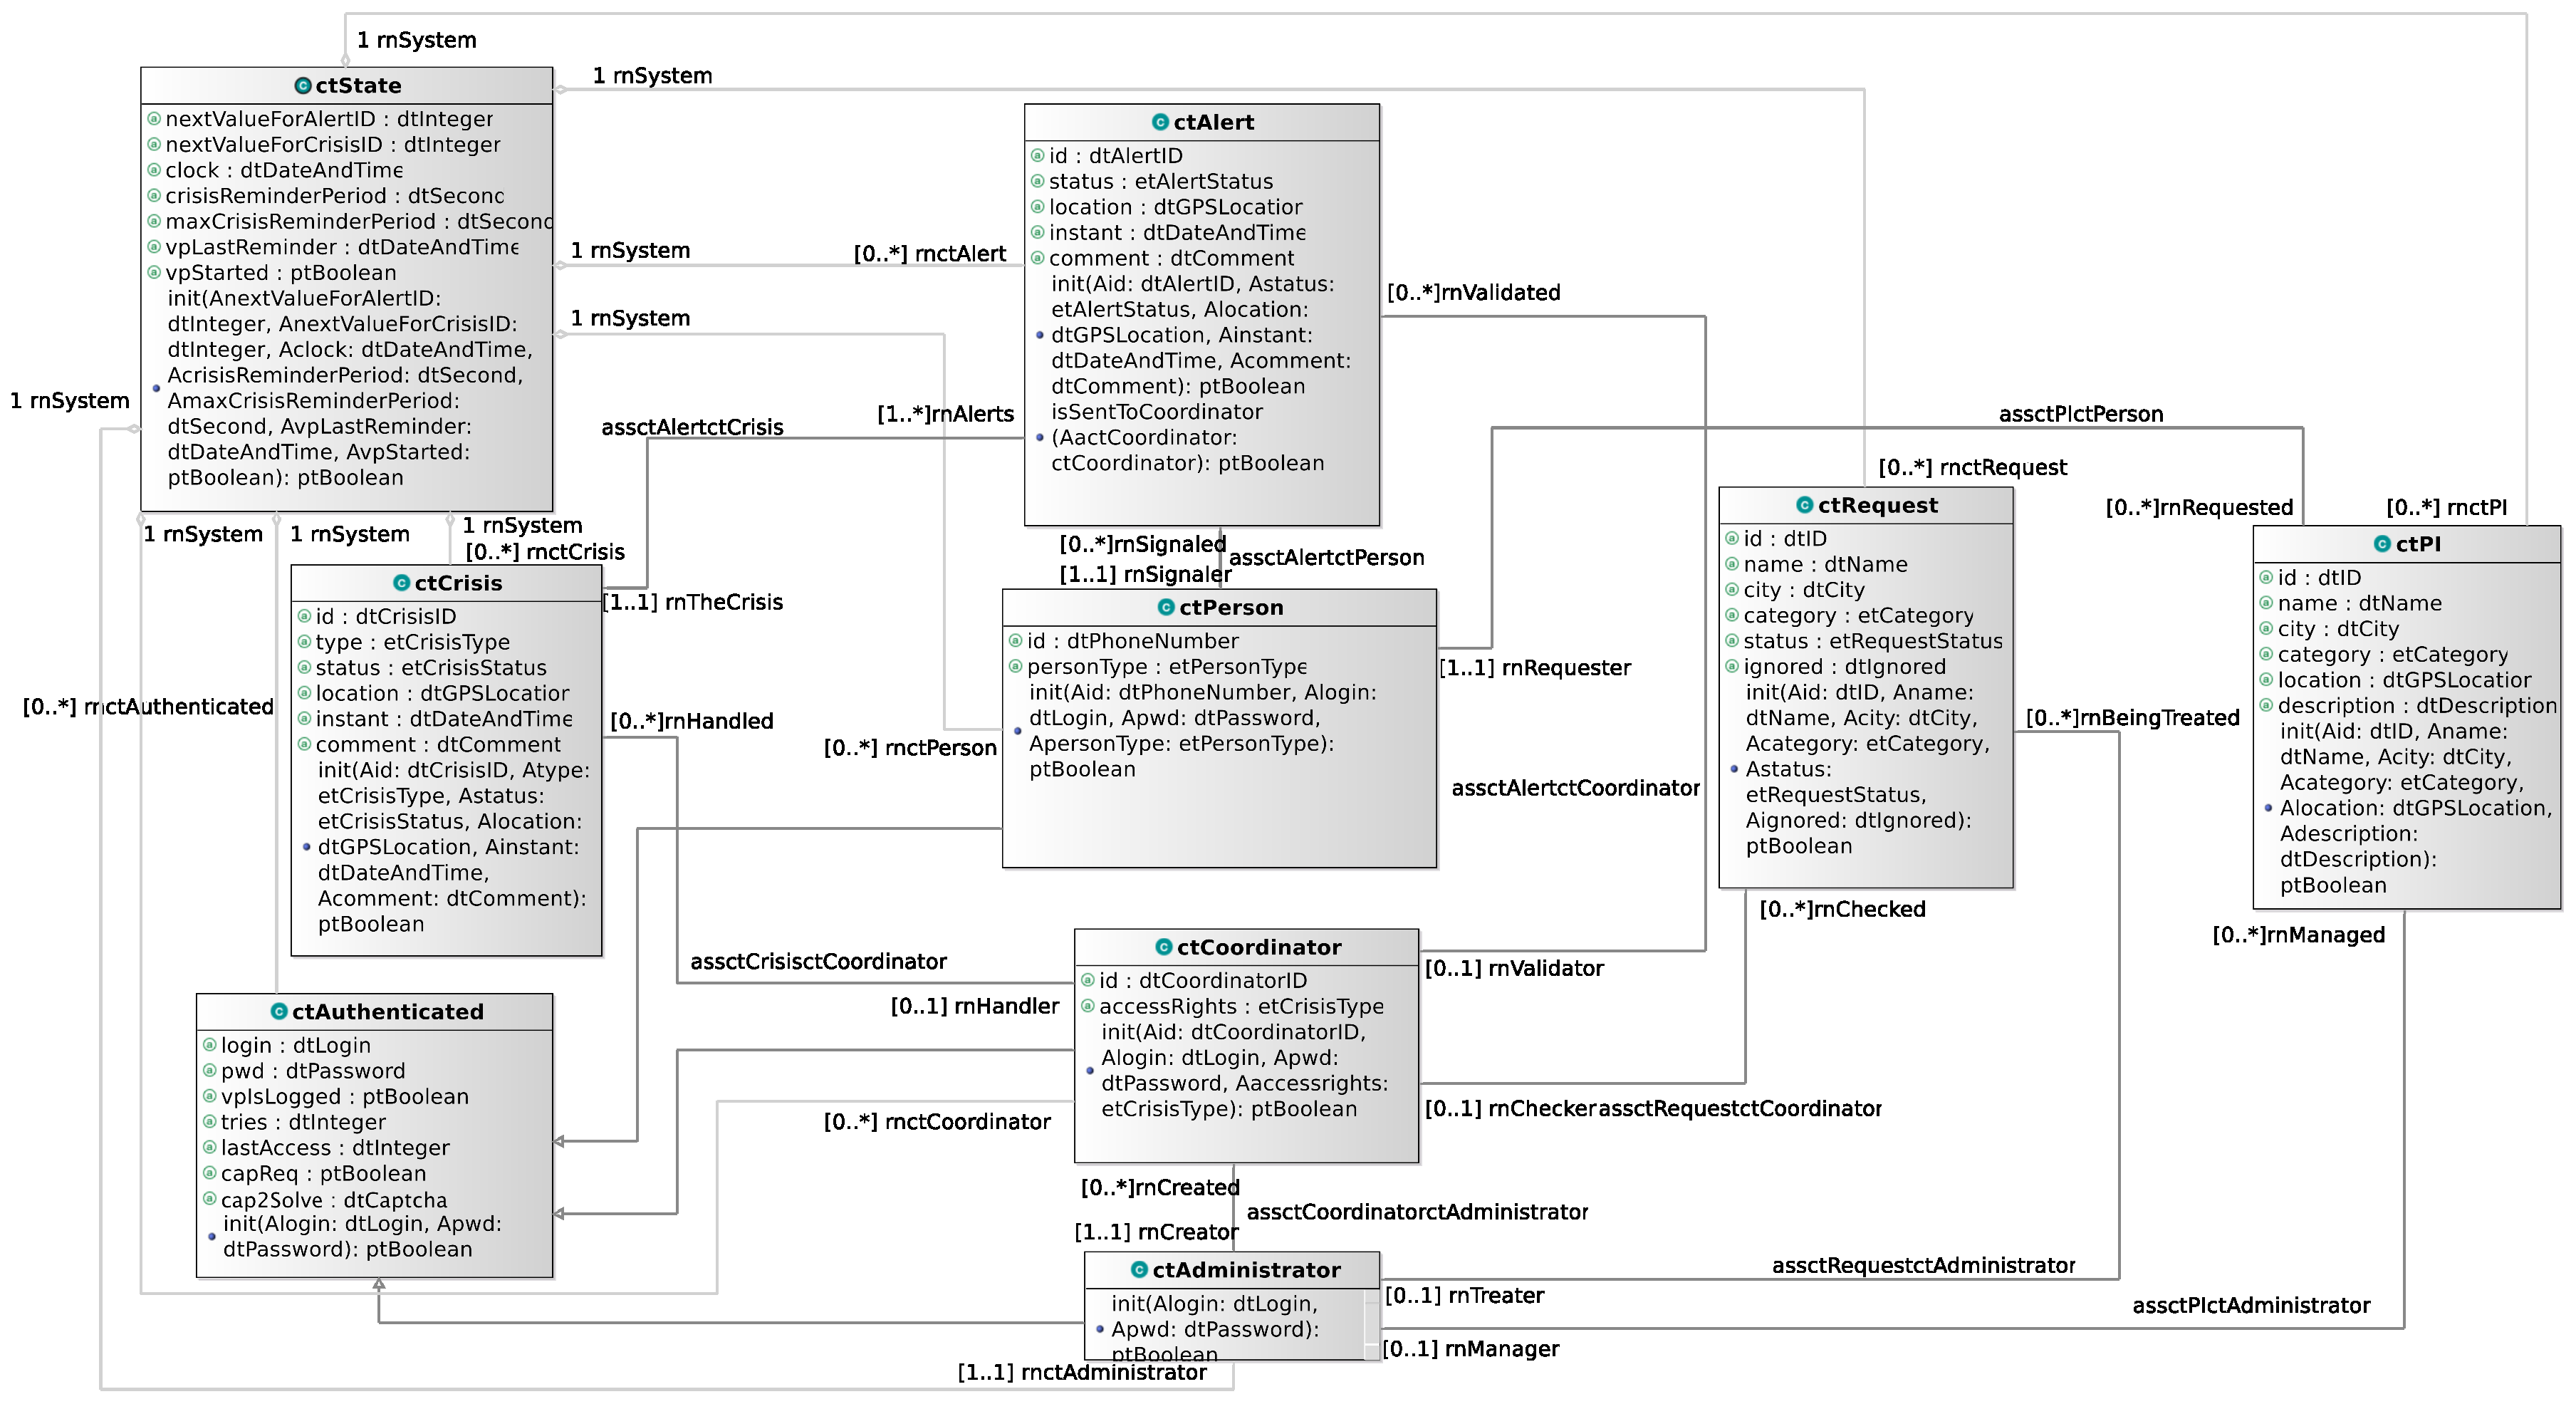
\includegraphics[
angle=0
,width=1.0\textwidth
]{./images-report-gen/concept-model/local/PrimaryTypes-Classes/01/PrimaryTypes-CLV-01.eps}
\end{center}
\caption[Concept Model - PrimaryTypes-Classes local view 01 - PrimaryTypes Classes local view 01]{Concept Model - PrimaryTypes-Classes local view 01. PrimaryTypes Classes local view 01.}
\label{fig:lu.uni.lassy.excalibur.MyCrash.G02-CM-view-local-PrimaryTypes-Classes-01}
\end{figure}
\vspace{0.5cm} 


\subsection{Global view 05}
\label{sec:lu.uni.lassy.excalibur.MyCrash.G02-CM-view-global-PrimaryTypes-Classes-05}
Figure \ref{fig:lu.uni.lassy.excalibur.MyCrash.G02-CM-view-global-PrimaryTypes-Classes-05} Represents class-actor relation for the PI variant



\begin{figure}[htbp] 
\label{fig:lu.uni.lassy.excalibur.MyCrash.G02-CM}
\begin{center}
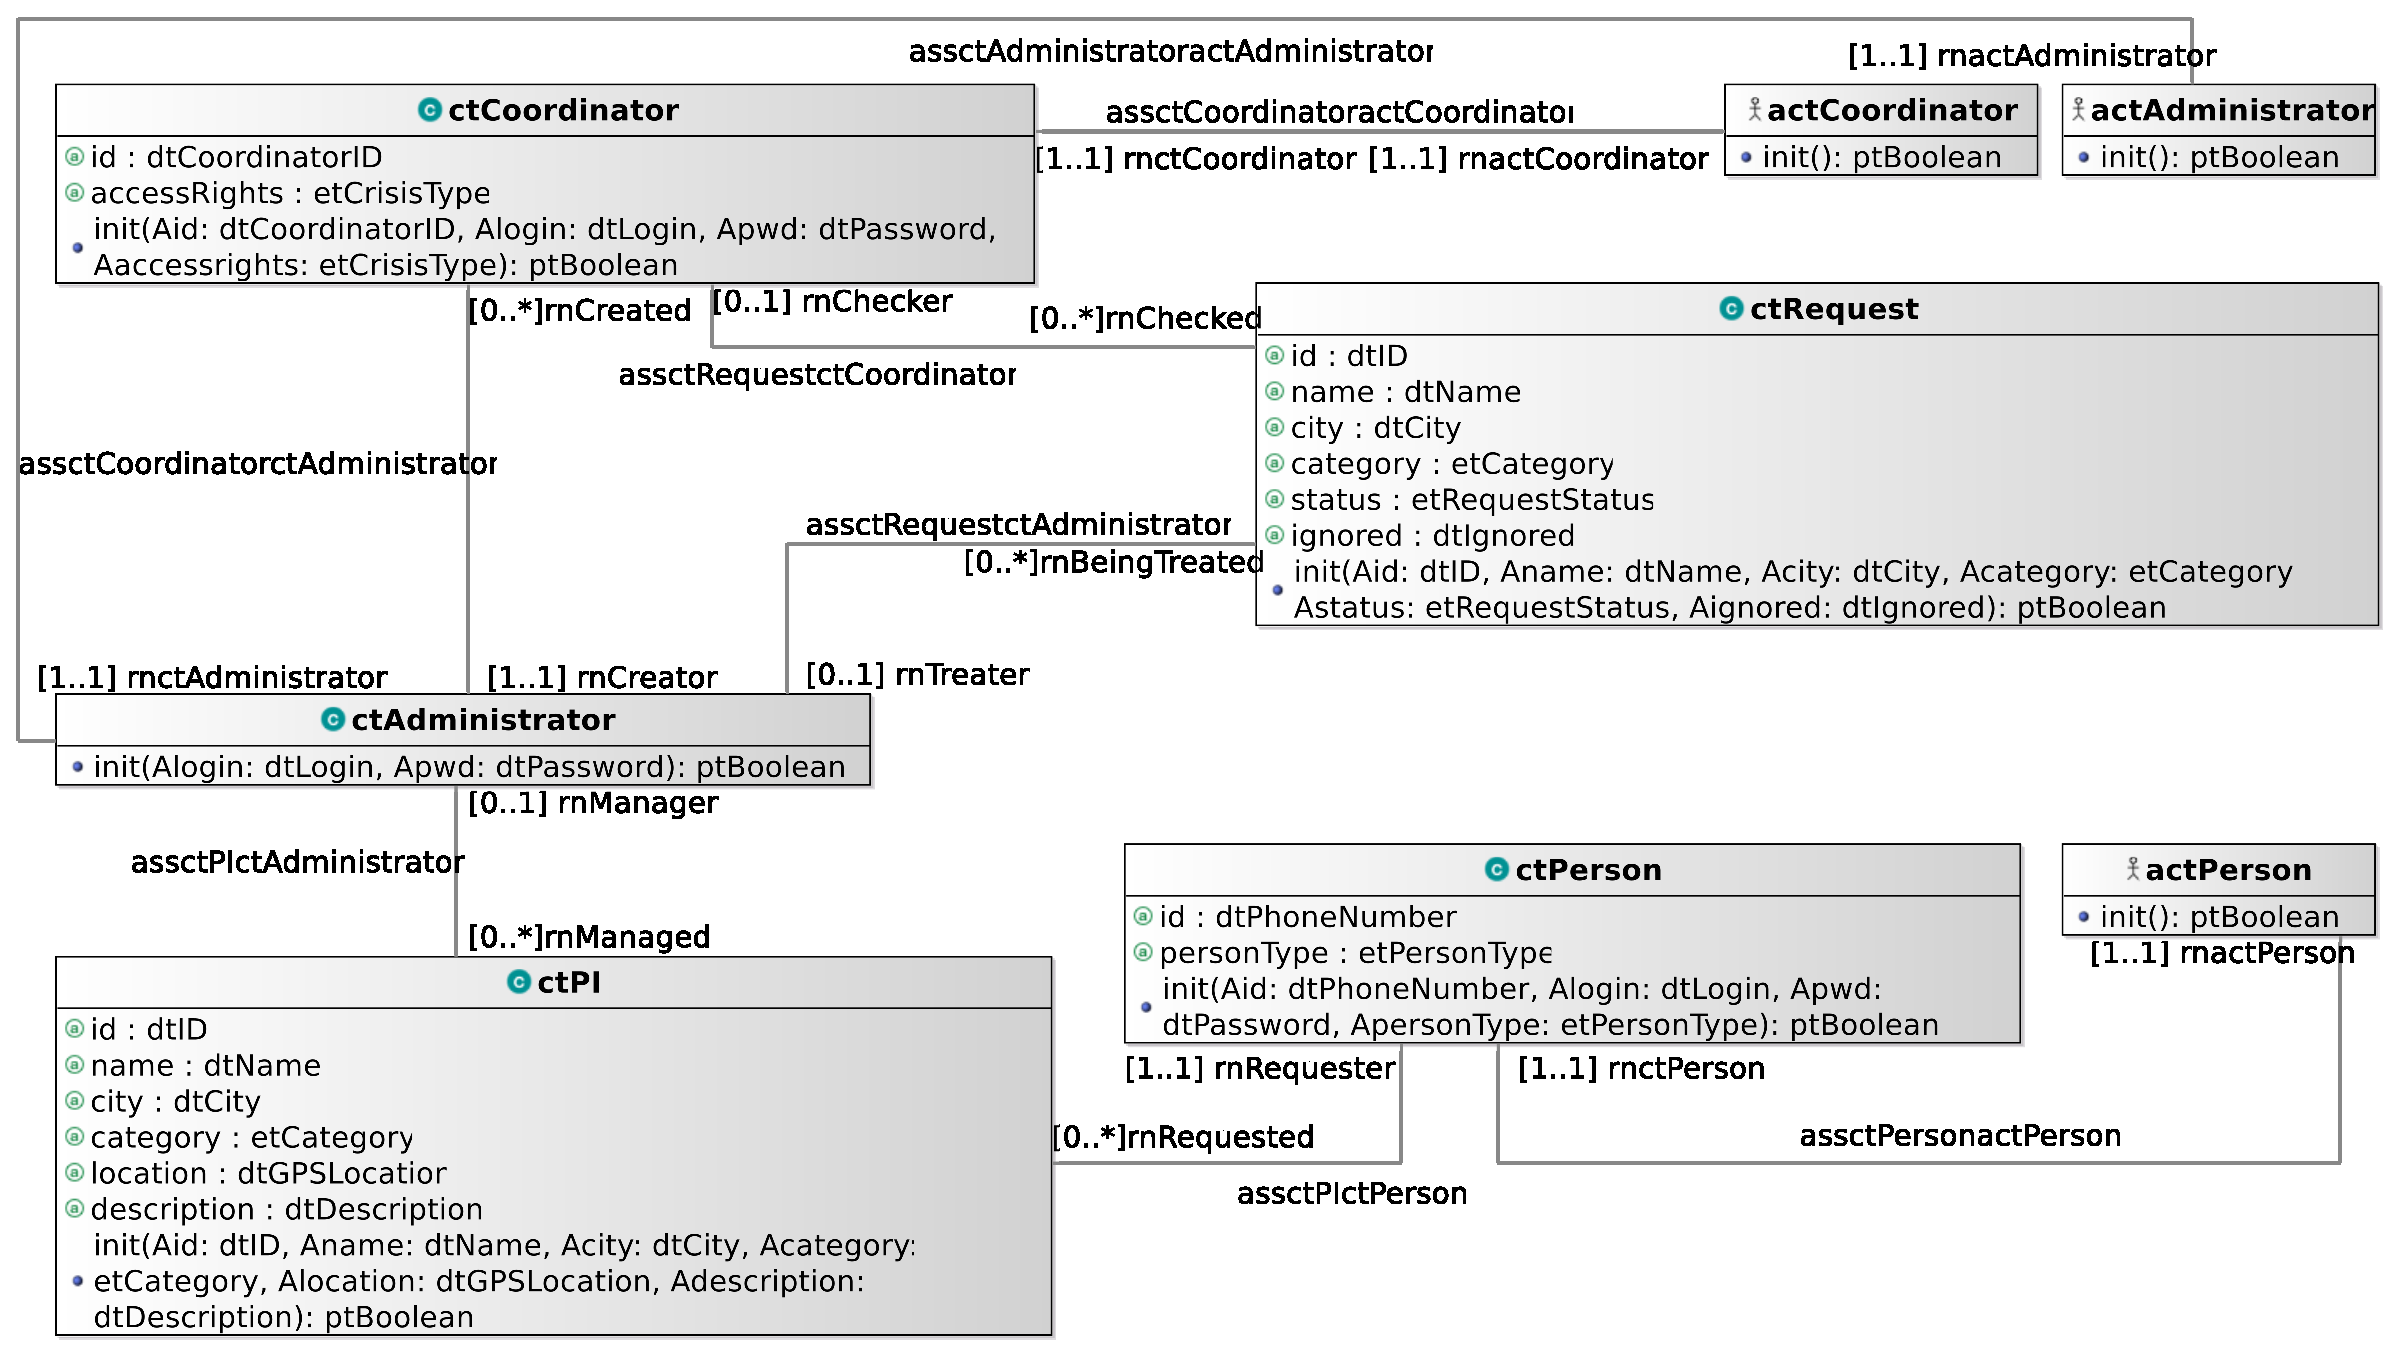
\includegraphics[
angle=0
,width=1.0\textwidth
]{./images-report-gen/concept-model/global/PrimaryTypes-Classes/05/PIvariant-CGV-01.eps}
\end{center}
\caption[Concept Model - PrimaryTypes-Classes global view 05 - PIvariant-CGV-01 concept global view]{Concept Model - PrimaryTypes-Classes global view 05. PIvariant-CGV-01 concept global view 01.}
\label{fig:lu.uni.lassy.excalibur.MyCrash.G02-CM-view-global-PrimaryTypes-Classes-05}
\end{figure}
\vspace{0.5cm} 

\subsection{Global view 06}
\label{sec:lu.uni.lassy.excalibur.MyCrash.G02-CM-view-global-PrimaryTypes-Classes-06}
Figure \ref{fig:lu.uni.lassy.excalibur.MyCrash.G02-CM-view-global-PrimaryTypes-Classes-06} Represents class and actor relation for Access Rights variant.



\begin{figure}[htbp] 
\label{fig:lu.uni.lassy.excalibur.MyCrash.G02-CM}
\begin{center}
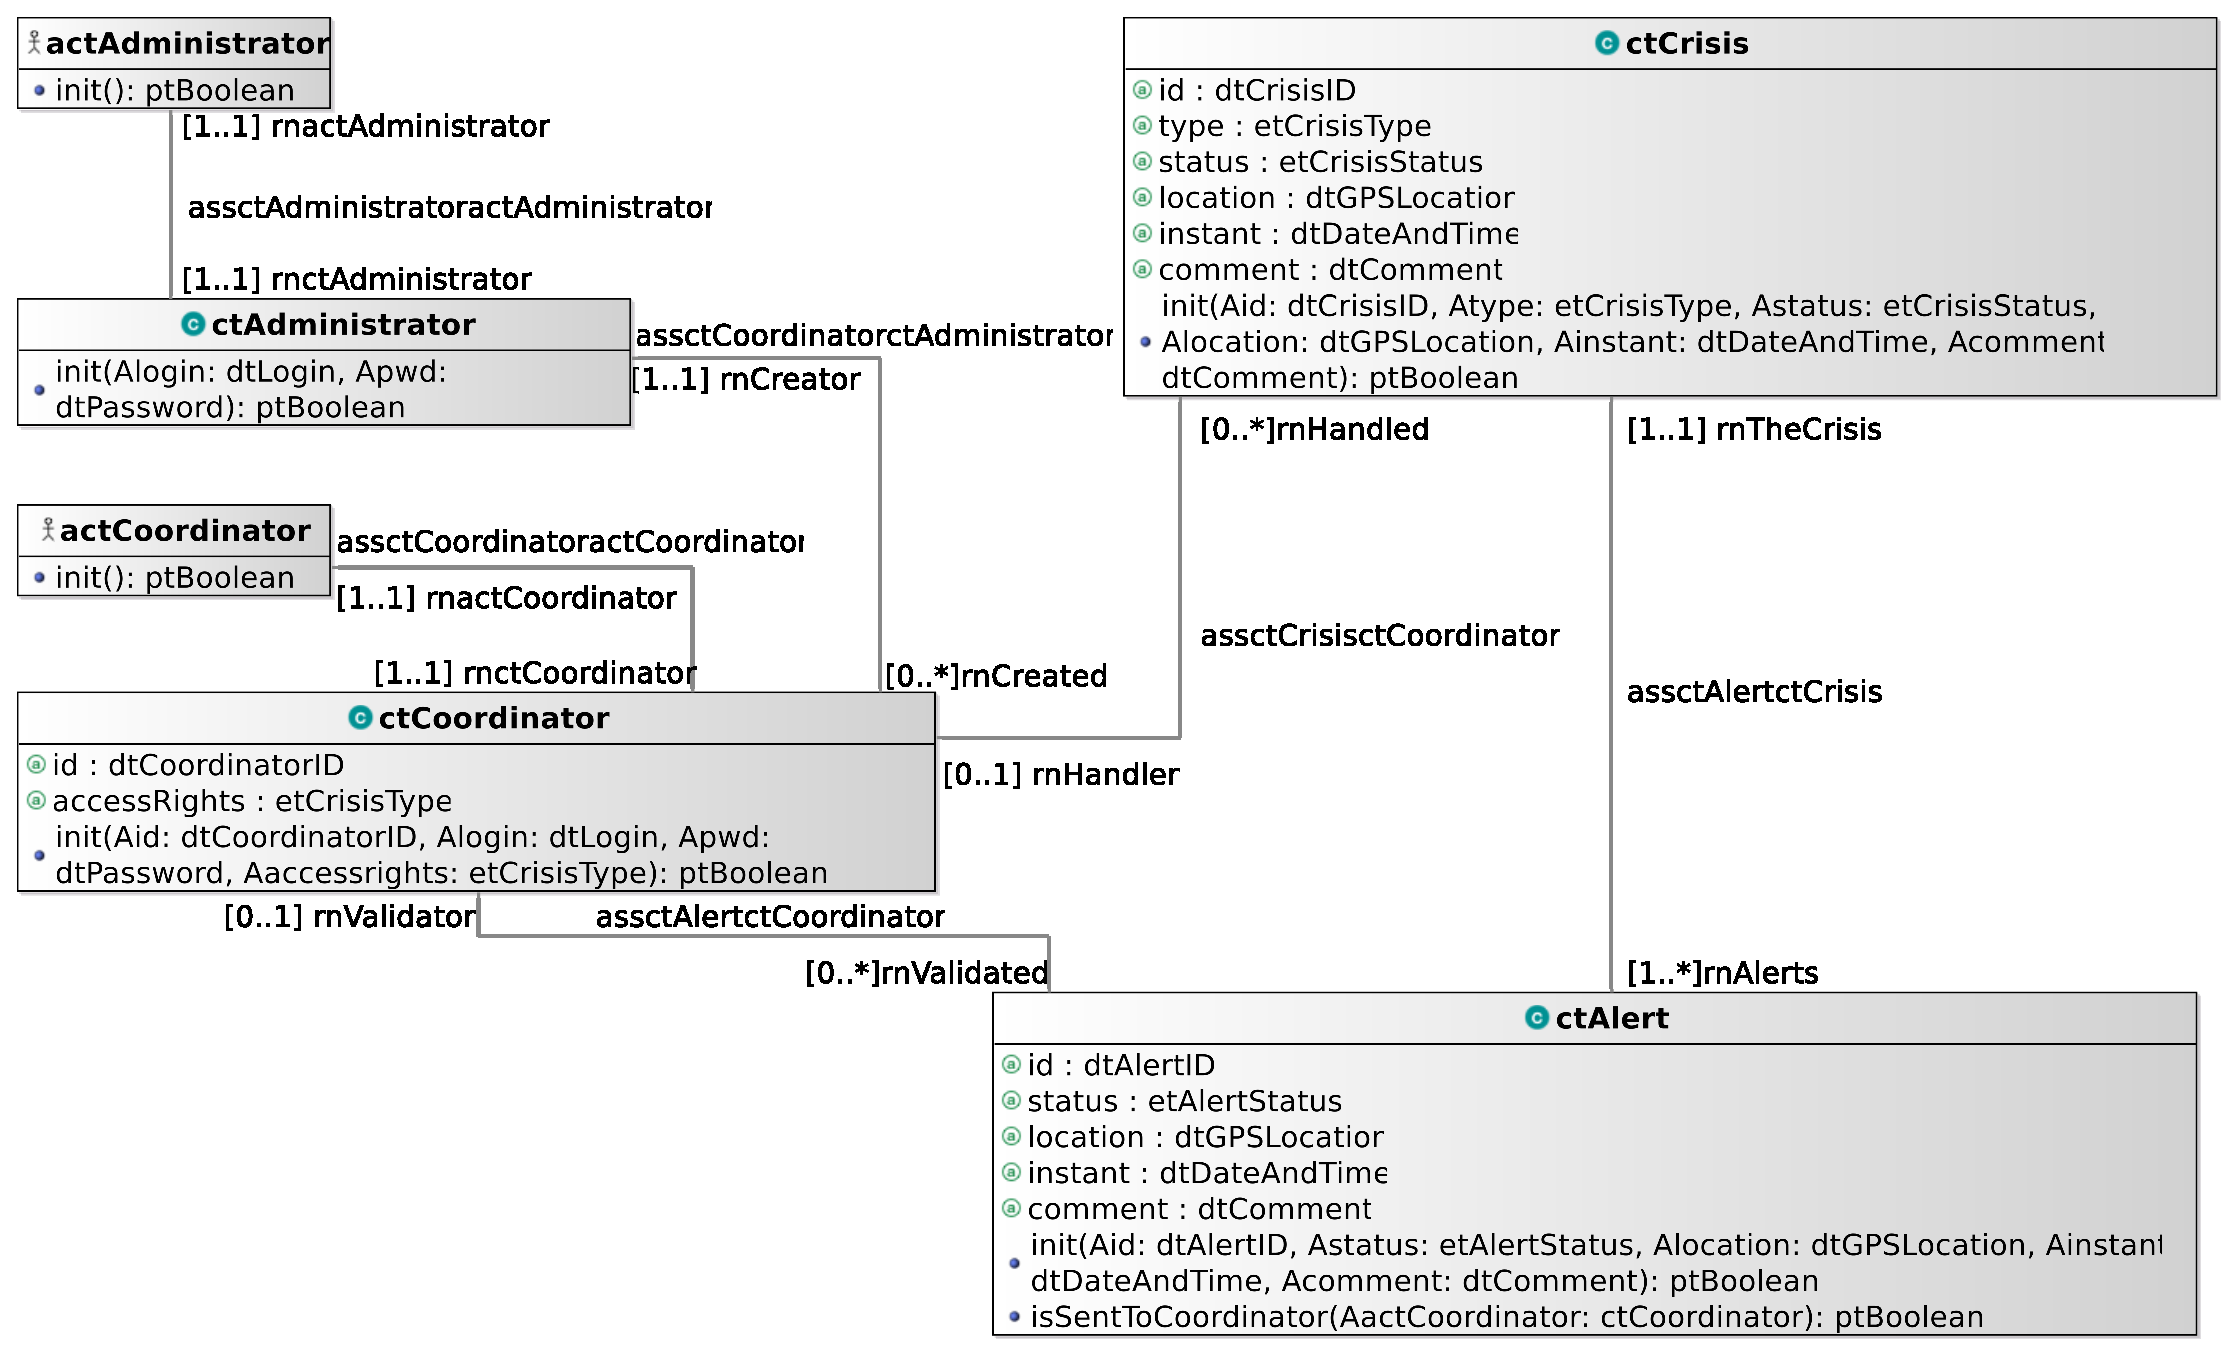
\includegraphics[
angle=0
]{./images-report-gen/concept-model/global/PrimaryTypes-Classes/06/ARvariant-CGV-01.eps}
\end{center}
\caption[Concept Model - PrimaryTypes-Classes global view 06 - ARvariant-CGV-01 concept global view]{Concept Model - PrimaryTypes-Classes global view 06. ARvariant-CGV-01 concept global view 01.}
\label{fig:lu.uni.lassy.excalibur.MyCrash.G02-CM-view-global-PrimaryTypes-Classes-06}
\end{figure}
\vspace{0.5cm} 











\section{Concept Model Types Descriptions}
This section provides the textual descriptions of all the types defined in the concept model and that can be part of the graphical views provided.

\subsection{Primary types - Class types descriptions}


There are no elements in this category in the system analysed.



\subsection{Primary types - Datatypes types descriptions}





The table below is providing comments on the graphical views given for the datatype types of the primary types.


\begin{datadictionary}
\addheading{Datatypes}

\adddoublerow{dtAdministratorID}{A string used to identify the administrator.}
\addsingletwocolumnrow{extends}{dtString}
\adddoubletwocolumnrow{operation}{\msrcode{is():ptBoolean}}{used to determine which strings are considered as valid administrator identifiers.}
\adddoublerow{dtAlertID}{A string used to identify alerts.}
\addsingletwocolumnrow{extends}{dtString}
\adddoubletwocolumnrow{operation}{\msrcode{is():ptBoolean}}{used to determine which strings are considered as valid alert identifiers.}
\adddoublerow{dtCaptcha}{A string used to store the Captcha information after the iCrash user failed to log in 
three times.}
\addsingletwocolumnrow{extends}{dtString}
\adddoubletwocolumnrow{operation}{\msrcode{is():ptBoolean}}{used to determine which strings are considered as valid dtCaptcha.}
\adddoublerow{dtCity}{A string used to store the name of the city in which the point of interest is situated.}
\addsingletwocolumnrow{extends}{dtString}
\adddoubletwocolumnrow{operation}{\msrcode{is():ptBoolean}}{used to determine which strings are considered as valid dtCity.}
\adddoublerow{dtComment}{A datatype made of a string value used to receive, store and send textual information 
about crisis and alerts.}
\addsingletwocolumnrow{extends}{dtString}
\adddoubletwocolumnrow{operation}{\msrcode{is():ptBoolean}}{used to determine which strings are considered as valid comments.}
\adddoublerow{dtCoordinatorID}{A string used to identify coordinators.}
\addsingletwocolumnrow{extends}{dtString}
\adddoubletwocolumnrow{operation}{\msrcode{is():ptBoolean}}{used to determine which strings are considered as valid coordinators identifiers.}
\adddoublerow{dtCrisisID}{A string used to identify crisis.}
\addsingletwocolumnrow{extends}{dtString}
\adddoubletwocolumnrow{operation}{\msrcode{is():ptBoolean}}{used to determine which strings are considered as valid crisis identifiers.}
\adddoublerow{dtDescription}{A datatype made of a string value used to receive, store and send textual information about 
a point of interest.}
\addsingletwocolumnrow{extends}{dtString}
\adddoubletwocolumnrow{operation}{\msrcode{is():ptBoolean}}{used to determine which strings are considered as valid descriptions.}
\adddoublerow{dtGPSLocation}{Used to define coordinates of geographical positions on earth. It is defined a couple made of a latitude
and a longitude.}
\addsingletwocolumnrow{extends}{dtString}
\adddoubletwocolumnrow{attribute}{\msrcode{latitude: dtLatitude}}{for the latitude part of the coordinate.}
\adddoubletwocolumnrow{attribute}{\msrcode{longitude: dtLongitude}}{for the longitude part of the coordinate.}
\adddoubletwocolumnrow{operation}{\msrcode{is():ptBoolean}}{used to determine which couples are considered as valid dtGPSLocation values.}
\adddoublerow{dtID}{A string used to identify points of interest and requests.}
\addsingletwocolumnrow{extends}{dtString}
\adddoubletwocolumnrow{operation}{\msrcode{is():ptBoolean}}{used to determine which strings are considered as valid points of interest and request identifiers.}
\adddoublerow{dtIgnored}{A boolean used to store the value considering if the request should be ignored or not.}
\adddoubletwocolumnrow{operation}{\msrcode{is():ptBoolean}}{used to determine which boolean values are considered as valid dtIgnored.}
\adddoublerow{dtLatitude}{Used to define a latitude value of a geographical positions on earth.}
\addsingletwocolumnrow{extends}{dtReal}
\adddoubletwocolumnrow{operation}{\msrcode{is():ptBoolean}}{used to determine which strings are considered as valid dtLatitude.}
\adddoublerow{dtLogin}{A login string used to authentify an iCrash user.}
\addsingletwocolumnrow{extends}{dtString}
\adddoubletwocolumnrow{operation}{\msrcode{is():ptBoolean}}{used to determine which strings are considered as valid dtLogin.}
\adddoublerow{dtLongitude}{Used to define a longitude value of a geographical positions on earth.}
\addsingletwocolumnrow{extends}{dtReal}
\adddoubletwocolumnrow{operation}{\msrcode{is():ptBoolean}}{used to determine which strings are considered as valid dtLongitude.}
\adddoublerow{dtMessage}{A string used to store the information that will be sent as input event to the actors.}
\addsingletwocolumnrow{extends}{dtString}
\adddoubletwocolumnrow{operation}{\msrcode{is():ptBoolean}}{used to determine which strings are considered as valid dtMessage.}
\adddoublerow{dtName}{A string used to store the names of the points of interest.}
\addsingletwocolumnrow{extends}{dtString}
\adddoubletwocolumnrow{operation}{\msrcode{is():ptBoolean}}{used to determine which strings are considered as valid names.}
\adddoublerow{dtPassword}{A password string used to authentify an iCrash user.}
\addsingletwocolumnrow{extends}{dtString}
\adddoubletwocolumnrow{operation}{\msrcode{is():ptBoolean}}{used to determine which strings are considered as valid dtPassword.}
\adddoublerow{dtPhoneNumber}{A string used to store the phone number from the person declaring the crisis or the alert.}
\addsingletwocolumnrow{extends}{dtString}
\adddoubletwocolumnrow{operation}{\msrcode{is():ptBoolean}}{used to determine which strings are considered as valid dtPhoneNumber.}
\end{datadictionary}


\begin{datadictionary}
\addheading{Enumerations}

\adddoublerow{etAlertStatus}{This type is used to indicate the different validation status of an alert.}
\adddoubletwocolumnrow{operation}{\msrcode{is():ptBoolean}}{used to determine which literal belongs to the enumeration.}
\adddoublerow{etCategory}{This type is used to indicate the different categories of a point of interest.}
\adddoubletwocolumnrow{operation}{\msrcode{is():ptBoolean}}{used to determine which literal belongs to the enumeration.}
\adddoublerow{etCrisisStatus}{This type is used to indicate the different handling status of a crisis.}
\adddoubletwocolumnrow{operation}{\msrcode{is():ptBoolean}}{used to determine which literal belongs to the enumeration.}
\adddoublerow{etCrisisType}{This type is used to indicate the different types of a crisis.}
\adddoubletwocolumnrow{operation}{\msrcode{is():ptBoolean}}{used to determine which literal belongs to the enumeration.}
\adddoublerow{etPersonType}{This type is used to indicate the type of person that informs about a car crash crisis.}
\adddoubletwocolumnrow{operation}{\msrcode{is():ptBoolean}}{used to determine which literal belongs to the enumeration.}
\adddoublerow{etRequestStatus}{This type is used to indicate the different status of the request made for a point of interest.}
\adddoubletwocolumnrow{operation}{\msrcode{is():ptBoolean}}{used to determine which literal belongs to the enumeration.}
\end{datadictionary}






\subsection{Primary types - Association types descriptions}




The table below is providing comments on the association types of the primary types.

\begin{associationtypes}
\addheading{Associations}
\adddoublerow{assctAdministratoractAdministrator}{frequent messages must be sent to coordinator especially in relation to coordinators they manage.}
\adddoublerow{assctAlertctCoordinator}{alerts need to be sent to coordinator in order to be validated or invalidated}
\adddoublerow{assctAlertctCrisis}{a crisis is related to one or more alerts as the alerts judged to concern all the same crisis due to their
location. An alert alerts exactly one crisis.}
\adddoublerow{assctAlertctPerson}{alerts are notified by person through the communication company. We need to keep an internal
representation of those person to allow for communication of alert handling.}
\adddoublerow{assctAuthenticatedactAuthenticated}{mainly used to determine if the login request of an authenticated actor can be granted based on the
given credentials and the registered ones.}
\adddoublerow{assctCoordinatoractCoordinator}{frequent messages must be sent to coordinator especially in relation to crisis they handle.}
\adddoublerow{assctCoordinatorctAdministrator}{one administrator manages more coordinators}
\adddoublerow{assctCrisisctCoordinator}{at any point in time we need to know if a coordinator is handling existing crisis or not.}
\adddoublerow{assctPersonactComCompany}{in order to communicate with person who informed about potential crisis, we need to record the
communication company to use to send them messages.}
\adddoublerow{assctPersonactPerson}{messages must be sent to person}
\adddoublerow{assctPIctAdministrator}{one administrator is charge of handling various point of interest}
\adddoublerow{assctPIctPerson}{several people can request several points of interests}
\adddoublerow{assctRequestctAdministrator}{one administrator is charge of handling various point of interest requests}
\adddoublerow{assctRequestctCoordinator}{several coordinators are charge of monitoring various point of interest requests}
\end{associationtypes}

\subsection{Primary types - Aggregation types descriptions}


There are no aggregation types for the primary types.


\subsubsection{Primary types - Composition types descriptions}



There are no composition types for the primary types.


\subsection{Secondary types - Class types descriptions}



There are no elements in this category in the system analysed.
		

\subsection{Secondary types - Datatypes types descriptions}





The table below is providing comments on the graphical views given for the datatype types of the secondary types.

\begin{datadictionary}
\addheading{Datatypes}

\adddoublerow{dtSMS}{A datatype made of a string value used to send textual information to human mobile devices.}
\adddoubletwocolumnrow{attribute}{\msrcode{value: ptString}}{the textual information.}
\adddoubletwocolumnrow{operation}{\msrcode{is():ptBoolean}}{used to determine which strings are considered as valid comments.}
\end{datadictionary}





\subsection{Secondary types - Association types descriptions}



There are no association types for the secondary types.



\subsection{Secondary types - Aggregation types descriptions}



There are no aggregation types for the secondary types.



\subsection{Secondary types - Composition types descriptions}



There are no composition types for the secondary types.





\chapter{Operation Model}
\label{chap:lu.uni.lassy.excalibur.standard.specification.libraries-OM}

This section contains the operation schemes of each operation defined in either an actor, its output interface, in a primary or secondary type (class, datatype or enumeration types). 
The \msrmessir OCL code listing is joined to the comment table.

\lstset{
float,
basicstyle=\scriptsize,
language=Messir,
breakatwhitespace=false,
tabsize=2,
breaklines=true,
numbers=left,
emptylines=1,
numbersep=5pt,
showspaces=false,
showstringspaces=false,
showtabs=false
} 


%% ***************************************************************
%% operations for: Environment-Out Interface Operation Schemes

\section{Environment - Out Interface Operation Schemes}
There are no elements in this category in the system analysed.
		

%% ***************************************************************
%% operations for: Environment-Actor Operation Schemes

\section{Environment - Actor Operation Schemes}
There are no elements in this category in the system analysed.
		

%% ***************************************************************
%% operations for primary type classes

\section{Primary Types - Operation Schemes for Classes}
There are no elements in this category in the system analysed.



%% ***************************************************************
%% operations for primary type datatypes and enumerations

\section{Primary Types - Operation Schemes for Datatypes}
There are no elements in this category in the system analysed.




\section{Primary Types - Operation Schemes for Enumerations}
There are no elements in this category in the system analysed.





%% ***************************************************************
%% operations for secondary type classes


\section{Secondary Types - Operation Schemes for Classes}
There are no elements in this category in the system analysed.




%% ***************************************************************
%% operations for secondary type datatypes and enumerations

\section{Secondary Types - Operation Schemes for Datatypes}
There are no elements in this category in the system analysed.



\section{Secondary Types - Operation Schemes for Enumerations}
There are no elements in this category in the system analysed.





\lstset{
float,
basicstyle=\scriptsize,
language=Messir,
breakatwhitespace=false,
tabsize=2,
breaklines=true,
numbers=left,
emptylines=1,
numbersep=5pt,
showspaces=false,
showstringspaces=false,
showtabs=false
} 

\chapter{Test Model(s)}
\label{chap:lu.uni.lassy.excalibur.MyCrash.G02-TM}

There are no elements in this category in the system analysed.








\newpage

% Last Modification:
% @author AUTHOR_NAME
% @date TODAY_DATE


\chapter{Additional Constraints}
\label{chap:additional_constraints}
\newpage

%APPENDICES
\appendix
% Last Modification:
% @author AUTHOR_NAME
% @date TODAY_DATE


%\chapter{AppendixName}
%\label{chap:AppendixName}




	
	\chapter{Messir Specification Files Listing}

\section[File /src-gen/messir-spec/.views.msr]{File ./src-gen/messir-spec/.views.msr}
\scriptsize
\lstinputlisting[style=MessirStyle,firstnumber=auto,captionpos=b,caption={Messir Spec. file .views.msr.}]{./src-gen/messir-spec/.views.msr}
\normalsize
	
\section[File /src-gen/messir-spec/library/calendar.msr]{File ./src-gen/messir-spec/library/calendar.msr}
\scriptsize
\lstinputlisting[style=MessirStyle,firstnumber=auto,captionpos=b,caption={Messir Spec. file calendar.msr.}]{./src-gen/messir-spec/library/calendar.msr}
\normalsize
	
\section[File /src-gen/messir-spec/library/math.msr]{File ./src-gen/messir-spec/library/math.msr}
\scriptsize
\lstinputlisting[style=MessirStyle,firstnumber=auto,captionpos=b,caption={Messir Spec. file math.msr.}]{./src-gen/messir-spec/library/math.msr}
\normalsize
	
\section[File /src-gen/messir-spec/library/primitives.msr]{File ./src-gen/messir-spec/library/primitives.msr}
\scriptsize
\lstinputlisting[style=MessirStyle,firstnumber=auto,captionpos=b,caption={Messir Spec. file primitives.msr.}]{./src-gen/messir-spec/library/primitives.msr}
\normalsize
	
\section[File /src-gen/messir-spec/library/string.msr]{File ./src-gen/messir-spec/library/string.msr}
\scriptsize
\lstinputlisting[style=MessirStyle,firstnumber=auto,captionpos=b,caption={Messir Spec. file string.msr.}]{./src-gen/messir-spec/library/string.msr}
\normalsize
	


	
	

\newpage

%GLOSSARY
\printglossaries
\newpage

%BIBLIOGRAPHY
\cleardoublepage
\bibliographystyle{./../lu.uni.lassy.excalibur.standard.report.libraries/styles/lncs} 
\bibliography{./../lu.uni.lassy.excalibur.standard.report.libraries/defs/references/messir,doc/bibliography/report}
\label{sec:references}

\end{document}
